\documentclass[12pt,a4paper]{article}

% ------------------------------------------------------------
% KÓDOLÁS, NYELV, BETŰKÉP
% ------------------------------------------------------------
\usepackage[T1]{fontenc}
\usepackage[utf8]{inputenc}
\usepackage[magyar]{babel}
\usepackage{lmodern}
\usepackage{microtype}

% ------------------------------------------------------------
% OLDALBEÁLLÍTÁS
% ------------------------------------------------------------
\usepackage[
a4paper,
left=25mm,
right=25mm,
top=25mm,
bottom=25mm
]{geometry}

% ------------------------------------------------------------
% MATEMATIKA ÉS MÉRTÉKEGYSÉGEK
% ------------------------------------------------------------
\usepackage{amsmath}
\usepackage{amssymb}
\usepackage{mathtools}
\setcounter{MaxMatrixCols}{20}
\usepackage{bm}
\usepackage{siunitx}
\sisetup{output-decimal-marker={,}}

% ------------------------------------------------------------
% TÁBLÁZATOK, LISTÁK
% ------------------------------------------------------------
\usepackage{booktabs}
\usepackage{longtable}
\usepackage{array}
\usepackage{enumitem}

% ------------------------------------------------------------
% ÁBRÁK ÉS BLOKKVÁZLATOK
% ------------------------------------------------------------
\usepackage{tikz}
\usetikzlibrary{arrows.meta,positioning,calc,shapes.geometric}
\usepackage{float}

% ------------------------------------------------------------
% KÓDRÉSZLETEK
% ------------------------------------------------------------
\usepackage{xcolor}
\usepackage{listings}
\lstdefinestyle{matlab}{
	language=Matlab,
	basicstyle=\ttfamily\small,
	keywordstyle=\bfseries,
	commentstyle=\itshape,
	showstringspaces=false,
	breaklines=true,
	frame=single,
	columns=fullflexible
}

% ------------------------------------------------------------
% HIVATKOZÁSOK
% ------------------------------------------------------------
\usepackage[hidelinks]{hyperref}

% ------------------------------------------------------------
% SAJÁT PARANCSOK
% ------------------------------------------------------------
\newcommand{\mbody}{m_{\mathrm{b}}}
\newcommand{\mwheel}{m_{\mathrm{w}}}
\newcommand{\Jspin}{J_{\mathrm{a}}}
\newcommand{\Jzw}{J_{z,\mathrm{w}}}
\newcommand{\tauL}{\tau_{\mathrm{L}}}
\newcommand{\tauR}{\tau_{\mathrm{R}}}
\newcommand{\tauc}{\tau_{\mathrm{c}}}
\newcommand{\taud}{\tau_{\mathrm{d}}}
\newcommand{\phiL}{\varphi_{\mathrm{L}}}
\newcommand{\phiR}{\varphi_{\mathrm{R}}}
\newcommand{\omegaL}{\omega_{\mathrm{L}}}
\newcommand{\omegaR}{\omega_{\mathrm{R}}}
\newcommand{\alphL}{\alpha_{\mathrm{L}}}
\newcommand{\alphR}{\alpha_{\mathrm{R}}}
\newcommand{\thetad}{\dot{\theta}}
\newcommand{\thetadd}{\ddot{\theta}}
\newcommand{\psid}{\dot{\psi}}
\newcommand{\psidd}{\ddot{\psi}}

\title{Kétkerekű, önkiegyensúlyozó, irányszög-szabályozásra képes mobil robot\\
	\large A mechanikai modell részletes levezetése és Simulink-felépítése}
\author{Várkonyi Borisz}
\date{2026}

\begin{document}
	
	\maketitle
	\tableofcontents
	\newpage
	
	% ============================================================
	\section{A modell célja}
	% ============================================================
	
	Ennek a fejezetnek kizárólag a robot \textbf{mechanikai modellje} a tárgya. Nem építünk még PID-, LQR- vagy megerősítéses tanulás alapú szabályozót, és nem foglalkozunk részletes szenzormodellel sem. A cél egy olyan nemlineáris mechanikai rendszer felépítése, amely a későbbi szabályozók közös fizikai modellje lehet.
	
	A robot két, egymástól függetlenül hajtott, közös tengelyvonalon elhelyezett kerékkel rendelkezik. A főtest a keréktengely fölött helyezkedik el, ezért a függőleges helyzet gravitációsan instabil: ha a test kissé előre vagy hátra billen, vezérlés nélkül tovább fog dőlni.
	
	A modellnek egyszerre kell leírnia:
	\begin{itemize}[leftmargin=2em]
		\item a robot előre--hátra haladását;
		\item a főtest előre--hátra dőlését;
		\item a robot függőleges tengely körüli elfordulását;
		\item a két kerék gördülését;
		\item a dőlési és elfordulási mozgás közötti nemlineáris kölcsönhatásokat.
	\end{itemize}
	
	A modell első változatában a talajt merevnek és síknak tekintjük, a kerekek nem csúsznak sem hosszirányban, sem oldalirányban, a robot geometriailag szimmetrikus, a két kerék azonos, és a főtest merev testként viselkedik. A részletes érintkezési, súrlódási és csúszási jelenségek később Simscape Multibody modellben vizsgálhatók.
	
	% ============================================================
	\section{Koordinátarendszer és előjel-konvenció}
	% ============================================================
	
	Minden további egyenlet csak akkor marad következetes, ha a koordinátarendszert és az előjeleket már az elején rögzítjük.
	
	A világkoordináta-rendszer jobbkezes:
	\begin{align*}
		X &: \text{előre},\\
		Y &: \text{balra},\\
		Z &: \text{felfelé}.
	\end{align*}
	
	A robot helyzetét és orientációját a következő mennyiségekkel írjuk le:
	\begin{itemize}[leftmargin=2em]
		\item $x$: a keréktengely középpontjának $X$ koordinátája;
		\item $y$: a keréktengely középpontjának $Y$ koordinátája;
		\item $\psi$: a robot irányszöge a függőleges tengely körül;
		\item $\theta$: a főtest hosszirányú dőlésszöge;
		\item $\phiL$: a bal kerék talajhoz viszonyított abszolút gördülési szöge;
		\item $\phiR$: a jobb kerék talajhoz viszonyított abszolút gördülési szöge.
	\end{itemize}
	
	Az előjel-konvenció:
	\begin{itemize}[leftmargin=2em]
		\item $\theta>0$: a főtest teteje előrefelé dől;
		\item $\psi>0$: felülről nézve a robot balra fordul, vagyis pozitív $Z$ tengely körüli elfordulás történik.
	\end{itemize}
	
	A teljes konfigurációs vektor így:
	\begin{equation}
		\bm q_{\mathrm{teljes}}=
		\begin{bmatrix}
			x & y & \psi & \theta & \phiL & \phiR
		\end{bmatrix}^{\!T}.
	\end{equation}
	
	Fontos: ez a hat koordináta \textbf{nem hat egymástól független szabadságfok}. A gördülési kényszerek összekapcsolják őket.
	
	% ============================================================
	\section{A modell fizikai paraméterei}
	% ============================================================
	
	\begin{longtable}{>{\centering\arraybackslash}p{2.5cm} p{8cm} p{2.5cm}}
		\toprule
		\textbf{Jel} & \textbf{Jelentés} & \textbf{Egység} \\
		\midrule
		\endfirsthead
		\toprule
		\textbf{Jel} & \textbf{Jelentés} & \textbf{Egység} \\
		\midrule
		\endhead
		$\mbody$ & a főtest tömege & \si{kg} \\
		$\mwheel$ & egy kerék tömege & \si{kg} \\
		$r$ & keréksugár & \si{m} \\
		$b$ & nyomtáv, vagyis a két kerék érintkezési síkja közötti távolság & \si{m} \\
		$l$ & a keréktengely és a főtest tömegközéppontja közötti távolság & \si{m} \\
		$I_x$ & a főtest tehetetlenségi nyomatéka a test $x$ tengelye körül & \si{kg.m^2} \\
		$I_y$ & a főtest tehetetlenségi nyomatéka a test $y$ tengelye körül & \si{kg.m^2} \\
		$I_z$ & a főtest tehetetlenségi nyomatéka a test $z$ tengelye körül & \si{kg.m^2} \\
		$\Jspin$ & egy kerék tengelyirányú forgási tehetetlensége & \si{kg.m^2} \\
		$\Jzw$ & egy kerék elfordulási mozgáshoz tartozó tehetetlensége & \si{kg.m^2} \\
		$g$ & gravitációs gyorsulás & \si{m.s^{-2}} \\
		$\tauL$ & bal kerék kerékoldali hajtónyomatéka & \si{N.m} \\
		$\tauR$ & jobb kerék kerékoldali hajtónyomatéka & \si{N.m} \\
		\bottomrule
	\end{longtable}
	
	% ============================================================
	\section{Miért nem használjuk közvetlenül a hat koordinátát?}
	% ============================================================
	
	Ha a kerekek csúszás nélkül gördülnek, akkor a robot síkbeli helyzete, irányszöge és kerékfordulatai nem változhatnak egymástól függetlenül.
	
	Például ha mindkét kerék áll, akkor a robot nem haladhat előre. Ha a jobb kerék gyorsabban forog, mint a bal, akkor a robotnak fordulnia kell. Emiatt a mozgást kényszeregyenletek kapcsolják össze.
	
	A mechanikai dinamika szempontjából célszerű a következő redukált koordinátákat használni:
	\begin{equation}
		\bm q_r=
		\begin{bmatrix}
			s\\
			\theta\\
			\psi
		\end{bmatrix},
	\end{equation}
	
	ahol $s$ a robot saját hosszirányában megtett út.
	
	A sebességvektor:
	\begin{equation}
		\dot{\bm q}_r=
		\begin{bmatrix}
			\dot s\\
			\dot\theta\\
			\dot\psi
		\end{bmatrix}
		=
		\begin{bmatrix}
			v\\
			\dot\theta\\
			\dot\psi
		\end{bmatrix}.
	\end{equation}
	
	Tehát:
	\begin{itemize}[leftmargin=2em]
		\item $v$ a robot előremeneti sebessége;
		\item $\dot\theta$ a főtest dőlési szögsebessége;
		\item $\dot\psi$ a robot elfordulási szögsebessége.
	\end{itemize}
	
	A világkoordinátás $x$ és $y$ helyzetet később külön, kinematikai összefüggésekkel számítjuk ki.
	
	% ============================================================
	\section{Síkbeli kinematika}
	% ============================================================
	
	\subsection{A robot előre- és balirányú egységvektora}
	
	A robot irányszöge $\psi$. A saját előreirányú egységvektora a világkoordináta-rendszerben:
	\begin{equation}
		\bm e_f=
		\begin{bmatrix}
			\cos\psi\\
			\sin\psi\\
			0
		\end{bmatrix}.
	\end{equation}
	
	A robot balirányú egységvektora:
	\begin{equation}
		\bm e_l=
		\begin{bmatrix}
			-\sin\psi\\
			\cos\psi\\
			0
		\end{bmatrix}.
	\end{equation}
	
	A keréktengely középpontjának világkoordinátás sebessége:
	\begin{equation}
		\bm v_P=
		\begin{bmatrix}
			\dot x\\
			\dot y\\
			0
		\end{bmatrix}.
	\end{equation}
	
	Ennek előreirányú komponense:
	\begin{equation}
		v=\bm e_f^T\bm v_P
		=\dot x\cos\psi+\dot y\sin\psi.
	\end{equation}
	
	Oldalirányú csúszás nélkül az oldalirányú sebesség nulla:
	\begin{equation}
		\bm e_l^T\bm v_P=0,
	\end{equation}
	
	vagyis:
	\begin{equation}
		-\dot x\sin\psi+\dot y\cos\psi=0.
	\end{equation}
	
	A két egyenletből közvetlenül adódik:
	\begin{align}
		\dot x &= v\cos\psi,\\
		\dot y &= v\sin\psi.
	\end{align}
	
	Ez lesz a Simulinkben a világkoordinátás helyzetet számító külön kinematikai rész.
	
	% ============================================================
	\section{A két kerék kinematikája}
	% ============================================================
	
	A bal és jobb kerék a robot középvonalától $b/2$ távolságban helyezkedik el.
	
	Ha a robot elfordulási szögsebessége $\dot\psi$, akkor a két kerék hosszirányú sebessége:
	\begin{align}
		v_L &= v-\frac{b}{2}\dot\psi,\\
		v_R &= v+\frac{b}{2}\dot\psi.
	\end{align}
	
	Csúszásmentes gördülés esetén:
	\begin{align}
		v_L &= r\dot\phiL,\\
		v_R &= r\dot\phiR.
	\end{align}
	
	Behelyettesítve:
	\begin{align}
		r\dot\phiL &= v-\frac{b}{2}\dot\psi,\\
		r\dot\phiR &= v+\frac{b}{2}\dot\psi.
	\end{align}
	
	A két egyenletet összeadva:
	\begin{equation}
		r(\dot\phiR+\dot\phiL)=2v,
	\end{equation}
	
	tehát:
	\begin{equation}
		\boxed{
			v=\frac{r}{2}(\dot\phiR+\dot\phiL)
		}
	\end{equation}
	
	A két egyenletet kivonva:
	\begin{equation}
		r(\dot\phiR-\dot\phiL)=b\dot\psi,
	\end{equation}
	
	tehát:
	\begin{equation}
		\boxed{
			\dot\psi=\frac{r}{b}(\dot\phiR-\dot\phiL)
		}
	\end{equation}
	
	Ha $\omega_L=\dot\phiL$ és $\omega_R=\dot\phiR$, akkor:
	\begin{align}
		\boxed{\omegaL=\frac{v-\frac{b}{2}\dot\psi}{r}},\\
		\boxed{\omegaR=\frac{v+\frac{b}{2}\dot\psi}{r}}.
	\end{align}
	
	% ============================================================
	\section{Abszolút kerékszög és a motorencoder szöge}
	% ============================================================
	
	A $\phiL$ és $\phiR$ mennyiségek a kerekek talajhoz, illetve világkoordinátához viszonyított abszolút gördülési szögei. Egy motorencoder azonban tipikusan a kereket a robot testéhez viszonyítva méri.
	
	Jelölje ezt a relatív szöget $\alpha_i$. A választott előjel-konvencióban:
	\begin{equation}
		\alpha_i=\phi_i-\theta.
	\end{equation}
	
	Így:
	\begin{equation}
		\dot\alpha_i=\dot\phi_i-\dot\theta.
	\end{equation}
	
	Konkrétan:
	\begin{align}
		\dot\alphL &= \omegaL-\dot\theta,\\
		\dot\alphR &= \omegaR-\dot\theta.
	\end{align}
	
	Ez később szenzormodellezésnél fontos, mert a nyers encodersebesség nem minden helyzetben azonos a talajhoz viszonyított keréksebességgel.
	
	% ============================================================
	\section{A főtest tömegközéppontjának helye}
	% ============================================================
	
	A keréktengely középpontját jelölje $P$. A főtest tömegközéppontja legyen $G$.
	
	A keréktengely középpontja:
	\begin{equation}
		\bm p_P=
		\begin{bmatrix}
			x\\y\\r
		\end{bmatrix}.
	\end{equation}
	
	A főtest tömegközéppontja a tengelytől $l$ távolságra van. A dőlési szög és az irányszög figyelembevételével:
	\begin{equation}
		\bm p_G=
		\begin{bmatrix}
			x\\y\\r
		\end{bmatrix}
		+l
		\begin{bmatrix}
			\sin\theta\cos\psi\\
			\sin\theta\sin\psi\\
			\cos\theta
		\end{bmatrix}.
	\end{equation}
	
	Ez azért lényeges, mert a főtest tömegközéppontja nem csupán előre--hátra mozog. Ha a robot dől és közben fordul, a tömegközéppont térbeli mozgása összetettebb lesz.
	
	% ============================================================
	\section{A főtest tömegközéppontjának sebessége}
	% ============================================================
	
	Az előző helyvektort idő szerint deriváljuk. A hosszirányú sebességet felhasználva:
	\begin{align}
		\dot x_G &= (v+l\cos\theta\,\dot\theta)\cos\psi
		-l\sin\theta\,\dot\psi\sin\psi,\\
		\dot y_G &= (v+l\cos\theta\,\dot\theta)\sin\psi
		+l\sin\theta\,\dot\psi\cos\psi,\\
		\dot z_G &= -l\sin\theta\,\dot\theta.
	\end{align}
	
	A sebesség négyzete egyszerűsítve:
	\begin{equation}
		\|\bm v_G\|^2
		=v^2
		+2lv\cos\theta\,\dot\theta
		+l^2\dot\theta^2
		+l^2\sin^2\theta\,\dot\psi^2.
	\end{equation}
	
	Ebben már jól látható két fontos fizikai jelenség:
	\begin{enumerate}[leftmargin=2em]
		\item a $2lv\cos\theta\,\dot\theta$ tag összekapcsolja az előremeneti és a dőlési mozgást;
		\item az $l^2\sin^2\theta\,\dot\psi^2$ tag miatt a fordulás és a dőlés sem teljesen független.
	\end{enumerate}
	
	% ============================================================
	\section{Közös és különbségi hajtónyomaték}
	% ============================================================
	
	A két fizikai motor nyomatékai:
	\begin{equation}
		\tauL,\qquad \tauR.
	\end{equation}
	
	A matematikai leírás szempontjából célszerű ezeket közös és különbségi összetevőre bontani:
	\begin{align}
		\boxed{\tauc=\frac{\tauL+\tauR}{2}},\\
		\boxed{\taud=\frac{\tauR-\tauL}{2}}.
	\end{align}
	
	Innen visszafelé:
	\begin{align}
		\boxed{\tauL=\tauc-\taud},\\
		\boxed{\tauR=\tauc+\taud}.
	\end{align}
	
	A közös nyomatékösszetevő mindkét kereket azonos irányban hajtja, ezért elsősorban az előremeneti és dőlési mozgást gerjeszti.
	
	A különbségi nyomatékösszetevő a két kerék közötti eltérést írja le, ezért elsősorban a függőleges tengely körüli elfordulást gerjeszti.
	
	% ============================================================
	\section{A hajtónyomatékok általánosított erői}
	% ============================================================
	
	A redukált koordinátákhoz tartozó általánosított erők a következők.
	
	\subsection{Előremeneti irány}
	
	A két kerék a talajon összesen olyan hosszanti hajtóhatást hoz létre, amely nyomatékból erőre a keréksugárral alakítható át:
	\begin{equation}
		Q_v=\frac{\tauL+\tauR}{r}
		=\frac{2\tauc}{r}.
	\end{equation}
	
	\subsection{Dőlési irány}
	
	Ha a motor pozitív nyomatékkal előre gyorsítja a kerekeket, a főtestre ellenkező irányú reakciónyomaték hat. Ezért:
	\begin{equation}
		Q_\theta=-(\tauL+\tauR)=-2\tauc.
	\end{equation}
	
	\subsection{Elfordulási irány}
	
	A két kerék hosszanti erejének különbsége a $b$ nyomtáv miatt elfordító nyomatékot hoz létre:
	\begin{equation}
		Q_\psi=\frac{b}{2r}(\tauR-\tauL)
		=\frac{b}{r}\taud.
	\end{equation}
	
	Ezekből később közvetlenül felépíthető a bemeneti mátrix.
	
	% ============================================================
	\section{A kinetikus energia felépítése}
	% ============================================================
	
	A Lagrange-módszerben a teljes kinetikus energia minden mozgó rész energia-hozzájárulásának összege.
	
	\subsection{A főtest transzlációs kinetikus energiája}
	
	\begin{equation}
		T_{b,t}=\frac{1}{2}\mbody\|\bm v_G\|^2.
	\end{equation}
	
	Az előzőleg kapott sebességnégyzet behelyettesítésével:
	\begin{equation}
		T_{b,t}=\frac{1}{2}\mbody
		\left(
		v^2
		+2lv\cos\theta\,\dot\theta
		+l^2\dot\theta^2
		+l^2\sin^2\theta\,\dot\psi^2
		\right).
	\end{equation}
	
	\subsection{A főtest forgási kinetikus energiája}
	
	A választott orientációban a főtest szögsebességének testkoordinátás komponensei:
	\begin{equation}
		\bm\omega_b=
		\begin{bmatrix}
			-\dot\psi\sin\theta\\
			\dot\theta\\
			\dot\psi\cos\theta
		\end{bmatrix}.
	\end{equation}
	
	Így a forgási kinetikus energia:
	\begin{equation}
		T_{b,r}=
		\frac{1}{2}I_y\dot\theta^2
		+
		\frac{1}{2}
		\left(I_x\sin^2\theta+I_z\cos^2\theta\right)
		\dot\psi^2.
	\end{equation}
	
	\subsection{A kerekek transzlációs kinetikus energiája}
	
	A két kerék középpontjának hosszirányú sebessége:
	\begin{align*}
		v_L &= v-\frac{b}{2}\dot\psi,\\
		v_R &= v+\frac{b}{2}\dot\psi.
	\end{align*}
	
	A két kerék transzlációs kinetikus energiája:
	\begin{equation}
		T_{w,t}=\frac{1}{2}\mwheel v_L^2+
		\frac{1}{2}\mwheel v_R^2.
	\end{equation}
	
	Kifejtve:
	\begin{equation}
		T_{w,t}=\mwheel v^2+\frac{1}{4}\mwheel b^2\dot\psi^2.
	\end{equation}
	
	\subsection{A kerekek saját tengely körüli forgási energiája}
	
	A kerék szögsebességek:
	\begin{align*}
		\omegaL &= \frac{v-\frac{b}{2}\dot\psi}{r},\\
		\omegaR &= \frac{v+\frac{b}{2}\dot\psi}{r}.
	\end{align*}
	
	Ezért:
	\begin{equation}
		T_{w,a}=\frac{1}{2}\Jspin\omegaL^2+
		\frac{1}{2}\Jspin\omegaR^2.
	\end{equation}
	
	Egyszerűsítve:
	\begin{equation}
		T_{w,a}=\frac{\Jspin}{r^2}v^2
		+\frac{\Jspin b^2}{4r^2}\dot\psi^2.
	\end{equation}
	
	\subsection{A kerekek elfordulási tehetetlensége}
	
	Ha egy kerék függőleges tengely körüli tehetetlensége $\Jzw$, akkor a két kerék együttes hozzájárulása:
	\begin{equation}
		T_{w,z}=\Jzw\dot\psi^2.
	\end{equation}
	
	% ============================================================
	\section{Összevont tehetetlenségi együtthatók}
	% ============================================================
	
	A teljes energia áttekinthetőbb alakjához három fontos mennyiséget vezetünk be.
	
	\subsection{Effektív hosszirányú tehetetlenség}
	
	\begin{equation}
		\boxed{
			A=\mbody+2\mwheel+\frac{2\Jspin}{r^2}
		}
	\end{equation}
	
	Az első két tag a főtest és a két kerék transzlációs tömeghatása, a $2\Jspin/r^2$ tag pedig a kerekek forgási tehetetlenségének hosszirányú mozgásra visszavetített hatása.
	
	\subsection{Effektív dőlési tehetetlenség}
	
	\begin{equation}
		\boxed{
			C=I_y+\mbody l^2
		}
	\end{equation}
	
	Az $I_y$ a főtest saját tömegközéppontja körüli tehetetlenség, a $\mbody l^2$ pedig a párhuzamos tengelyek tételéből származó hozzájárulás.
	
	\subsection{Effektív elfordulási tehetetlenség}
	
	\begin{equation}
		\boxed{
			\begin{aligned}
				D(\theta)=&\ I_x\sin^2\theta
				+I_z\cos^2\theta
				+\mbody l^2\sin^2\theta\\
				&+\frac{\mwheel b^2}{2}
				+\frac{\Jspin b^2}{2r^2}
				+2\Jzw.
			\end{aligned}
		}
	\end{equation}
	
	Ennek dőlési szög szerinti deriváltja:
	\begin{equation}
		\boxed{
			D'(\theta)
			=2\sin\theta\cos\theta
			\left(I_x-I_z+\mbody l^2\right)
		}
	\end{equation}
	
	% ============================================================
	\section{A teljes kinetikus energia redukált alakja}
	% ============================================================
	
	A korábbi részek összevonásával a teljes kinetikus energia:
	\begin{equation}
		\boxed{
			T=
			\frac{1}{2}Av^2
			+\mbody l\cos\theta\,v\dot\theta
			+\frac{1}{2}C\dot\theta^2
			+\frac{1}{2}D(\theta)\dot\psi^2
		}
	\end{equation}
	
	Ez az alak nagyon sok információt hordoz.
	
	\begin{itemize}[leftmargin=2em]
		\item $\tfrac12 Av^2$: az előremeneti mozgás energiája;
		\item $\mbody l\cos\theta\,v\dot\theta$: az előremeneti és dőlési mozgás közötti csatolás;
		\item $\tfrac12 C\dot\theta^2$: a dőlési mozgás energiája;
		\item $\tfrac12 D(\theta)\dot\psi^2$: az elfordulási mozgás energiája, amely maga is függ a dőlési szögtől.
	\end{itemize}
	
	% ============================================================
	\section{Potenciális energia}
	% ============================================================
	
	A főtest tömegközéppontjának magassága a keréktengelyhez képest:
	\begin{equation}
		h=l\cos\theta.
	\end{equation}
	
	Ezért a gravitációs potenciális energia, egy állandó tagtól eltekintve:
	\begin{equation}
		\boxed{
			V=\mbody g l\cos\theta
		}
	\end{equation}
	
	A $\theta=0$ helyzetben a potenciális energia maximális. Ez mutatja, hogy a függőleges helyzet instabil egyensúlyi pont.
	
	% ============================================================
	\section{A Lagrange-függvény}
	% ============================================================
	
	A Lagrange-függvény:
	\begin{equation}
		\boxed{
			L=T-V
		}
	\end{equation}
	
	tehát:
	\begin{equation}
		\begin{aligned}
			L=&\ \frac{1}{2}Av^2
			+\mbody l\cos\theta\,v\dot\theta
			+\frac{1}{2}C\dot\theta^2\\
			&+\frac{1}{2}D(\theta)\dot\psi^2
			-\mbody g l\cos\theta.
		\end{aligned}
	\end{equation}
	
	A gördülési és oldalirányú kényszerek eliminálása után a megengedett független sebességek:
	\begin{equation}
		v,\qquad \dot\theta,\qquad \dot\psi.
	\end{equation}
	
	% ============================================================
	\section{A nemlineáris mozgásegyenletek}
	% ============================================================
	
	A Lagrange--d'Alembert-egyenletek alkalmazása után a redukált rendszer három nemlineáris differenciálegyenlete adódik.
	
	\subsection{Előremeneti mozgás egyenlete}
	
	\begin{equation}
		\boxed{
			A\dot v
			+\mbody l\cos\theta\,\ddot\theta
			-\mbody l\sin\theta\,\dot\theta^2
			=\frac{2\tauc}{r}
		}
	\end{equation}
	
	Értelmezés:
	\begin{itemize}[leftmargin=2em]
		\item $A\dot v$: az előremeneti gyorsítás tehetetlenségi igénye;
		\item $\mbody l\cos\theta\,\ddot\theta$: a test szöggyorsulása visszahat az előremeneti mozgásra;
		\item $-\mbody l\sin\theta\,\dot\theta^2$: nemlineáris tehetetlenségi tag;
		\item $2\tauc/r$: a két motor közös nyomatékának előremeneti hatása.
	\end{itemize}
	
	\subsection{Dőlési mozgás egyenlete}
	
	\begin{equation}
		\boxed{
			\mbody l\cos\theta\,\dot v
			+C\ddot\theta
			-\frac{1}{2}D'(\theta)\dot\psi^2
			-\mbody g l\sin\theta
			=-2\tauc
		}
	\end{equation}
	
	Értelmezés:
	\begin{itemize}[leftmargin=2em]
		\item $\mbody l\cos\theta\,\dot v$: az alváz gyorsulása hat a dőlésre;
		\item $C\ddot\theta$: dőlési tehetetlenség;
		\item $-\tfrac12 D'(\theta)\dot\psi^2$: az elfordulási mozgás dőlésre gyakorolt nemlineáris hatása;
		\item $-\mbody g l\sin\theta$: gravitációs tag;
		\item $-2\tauc$: a kerék gyorsításakor a főtestre ható reakciónyomaték.
	\end{itemize}
	
	\subsection{Elfordulási mozgás egyenlete}
	
	\begin{equation}
		\boxed{
			D(\theta)\ddot\psi
			+D'(\theta)\dot\theta\dot\psi
			=\frac{b}{r}\taud
		}
	\end{equation}
	
	Értelmezés:
	\begin{itemize}[leftmargin=2em]
		\item $D(\theta)\ddot\psi$: elfordulási tehetetlenség;
		\item $D'(\theta)\dot\theta\dot\psi$: a dőlési és elfordulási mozgás közötti nemlineáris csatolás;
		\item $(b/r)\taud$: a két kerék nyomatékkülönbségének elfordító hatása.
	\end{itemize}
	
	% ============================================================
	\section{Mátrixos alak}
	% ============================================================
	
	A három egyenlet tömören:
	\begin{equation}
		\boxed{
			\bm M(\bm q_r)\ddot{\bm q}_r
			+\bm h(\bm q_r,\dot{\bm q}_r)
			=\bm B\bm u
		}
	\end{equation}
	
	ahol:
	\begin{equation}
		\bm u=
		\begin{bmatrix}
			\tauc\\
			\taud
		\end{bmatrix}.
	\end{equation}
	
	A gyorsulásvektor:
	\begin{equation}
		\ddot{\bm q}_r=
		\begin{bmatrix}
			\dot v\\
			\ddot\theta\\
			\ddot\psi
		\end{bmatrix}.
	\end{equation}
	
	A tömegmátrix:
	\begin{equation}
		\boxed{
			\bm M=
			\begin{bmatrix}
				A & \mbody l\cos\theta & 0\\
				\mbody l\cos\theta & C & 0\\
				0 & 0 & D(\theta)
			\end{bmatrix}
		}
	\end{equation}
	
	A nemlineáris tagokat összegyűjtő vektor:
	\begin{equation}
		\boxed{
			\bm h=
			\begin{bmatrix}
				-\mbody l\sin\theta\,\dot\theta^2\\
				-\frac{1}{2}D'(\theta)\dot\psi^2-\mbody g l\sin\theta\\
				D'(\theta)\dot\theta\dot\psi
			\end{bmatrix}
		}
	\end{equation}
	
	A bemeneti mátrix:
	\begin{equation}
		\boxed{
			\bm B=
			\begin{bmatrix}
				\frac{2}{r} & 0\\
				-2 & 0\\
				0 & \frac{b}{r}
			\end{bmatrix}
		}
	\end{equation}
	
	A numerikus számításhoz:
	\begin{equation}
		\ddot{\bm q}_r=
		\bm M^{-1}
		\left(
		\bm B\bm u-\bm h
		\right).
	\end{equation}
	
	MATLAB-ban azonban nem képezünk explicit inverzt. Ehelyett lineáris egyenletrendszert oldunk meg:
	\begin{equation}
		\boxed{
			\ddot{\bm q}_r
			=\bm M\backslash(\bm B\bm u-\bm h)
		}
	\end{equation}
	
	Ez numerikusan kedvezőbb és stabilabb.
	
	% ============================================================
	\section{Mit kell a Simulinkben ténylegesen kiszámolni?}
	% ============================================================
	
	A mechanikai modell bemenete:
	\begin{equation}
		\bm u=
		\begin{bmatrix}
			\tauc\\
			\taud
		\end{bmatrix}.
	\end{equation}
	
	A mechanikai állapotok:
	\begin{equation}
		\bm q_r=
		\begin{bmatrix}
			s\\
			\theta\\
			\psi
		\end{bmatrix},
		\qquad
		\dot{\bm q}_r=
		\begin{bmatrix}
			v\\
			\dot\theta\\
			\dot\psi
		\end{bmatrix}.
	\end{equation}
	
	A nemlineáris dinamika ezekből kiszámolja:
	\begin{equation}
		\ddot{\bm q}_r=
		\begin{bmatrix}
			\dot v\\
			\ddot\theta\\
			\ddot\psi
		\end{bmatrix}.
	\end{equation}
	
	Ezután két integrálási lépés szükséges:
	\begin{equation}
		\ddot{\bm q}_r
		\xrightarrow{\int}
		\dot{\bm q}_r
		\xrightarrow{\int}
		\bm q_r.
	\end{equation}
	
	% ============================================================
	\section{A Simulink mechanikai plant logikai felépítése}
	% ============================================================
	
	\begin{figure}[H]
		\centering
		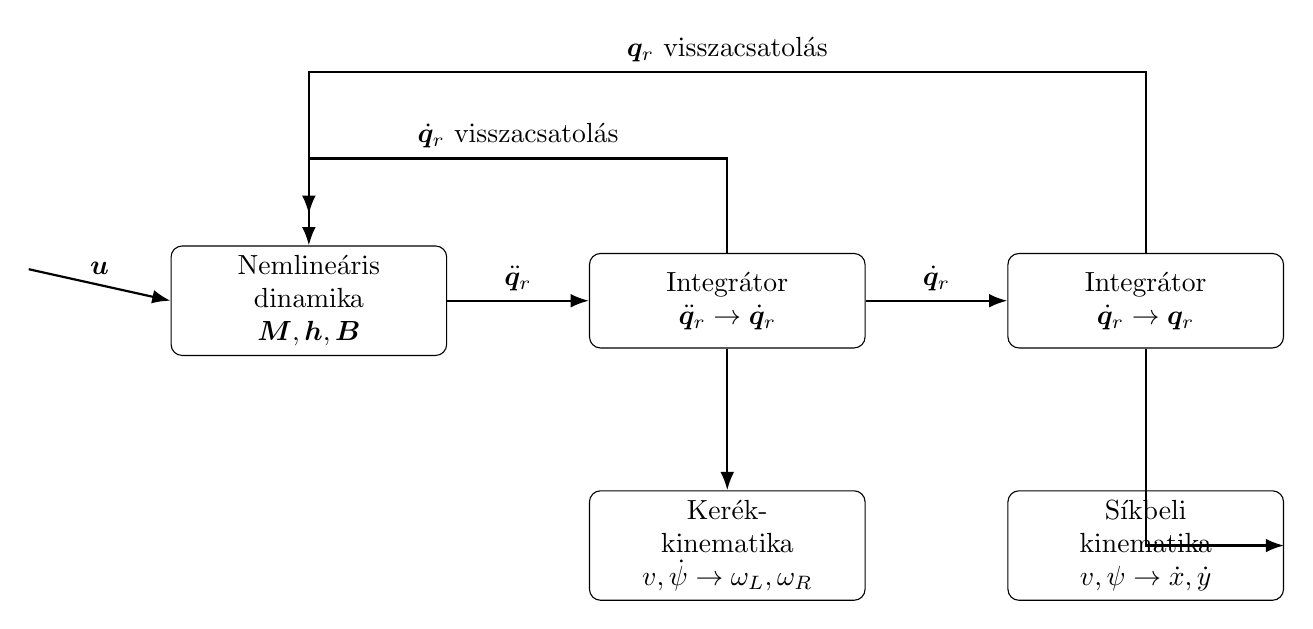
\begin{tikzpicture}[
			node distance=18mm,
			block/.style={draw, rounded corners, minimum width=35mm, minimum height=12mm, align=center},
			line/.style={-Latex, thick}
			]
			\node[block] (dyn) {Nemlineáris\\dinamika\\$\bm M,\bm h,\bm B$};
			\node[block, right=of dyn] (int1) {Integrátor\\$\ddot{\bm q}_r\to\dot{\bm q}_r$};
			\node[block, right=of int1] (int2) {Integrátor\\$\dot{\bm q}_r\to\bm q_r$};
			\node[block, below=of int2] (kin) {Síkbeli\\kinematika\\$v,\psi\to\dot x,\dot y$};
			\node[block, below=of int1] (wheel) {Kerék-\\kinematika\\$v,\dot\psi\to\omega_L,\omega_R$};
			
			\draw[line] ($(dyn.west)+(-18mm,4mm)$) -- node[above] {$\bm u$} (dyn.west);
			\draw[line] (dyn) -- node[above] {$\ddot{\bm q}_r$} (int1);
			\draw[line] (int1) -- node[above] {$\dot{\bm q}_r$} (int2);
			\draw[line] (int2.south) |- (kin.east);
			\draw[line] (int1.south) -- (wheel.north);
			\draw[line] (int1.north) |- ++(0,12mm) -| node[pos=0.25,above] {$\dot{\bm q}_r$ visszacsatolás} (dyn.north);
			\draw[line] (int2.north) |- ++(0,23mm) -| node[pos=0.25,above] {$\bm q_r$ visszacsatolás} ($(dyn.north)+(0,4mm)$);
		\end{tikzpicture}
		\caption{A mechanikai modell minimális Simulink-felépítése.}
	\end{figure}
	
	Fontos: a $\bm q_r$ és $\dot{\bm q}_r$ visszacsatolása itt nem szabályozási visszacsatolás. Erre azért van szükség, mert maga a differenciálegyenlet aktuális állapotfüggő.
	
	% ============================================================
	\section{A nemlineáris dinamika MATLAB Function blokkja}
	% ============================================================
	
	A Simulinkben hozzunk létre egy \texttt{MATLAB Function} blokkot, például \texttt{nonlinearDynamics} néven.
	
	Bemenetei:
	\begin{itemize}[leftmargin=2em]
		\item \texttt{q}: $[s,\theta,\psi]^T$;
		\item \texttt{qd}: $[v,\dot\theta,\dot\psi]^T$;
		\item \texttt{u}: $[\tau_c,\tau_d]^T$;
		\item \texttt{p}: a fizikai paraméterek vektora.
	\end{itemize}
	
	Kimenete:
	\begin{itemize}[leftmargin=2em]
		\item \texttt{qdd}: $[\dot v,\ddot\theta,\ddot\psi]^T$.
	\end{itemize}
	
	\begin{lstlisting}[style=matlab,caption={A nemlineáris mechanikai dinamika MATLAB Function blokkja}]
		function qdd = nonlinearDynamics(q, qd, u, p)
		% q  = [s; theta; psi]
		% qd = [v; thetaDot; psiDot]
		% u  = [tauCommon; tauDifferential]
		
		mb  = p(1);
		mw  = p(2);
		r   = p(3);
		b   = p(4);
		l   = p(5);
		Ix  = p(6);
		Iy  = p(7);
		Iz  = p(8);
		Ja  = p(9);
		Jzw = p(10);
		g   = p(11);
		
		theta    = q(2);
		thetaDot = qd(2);
		psiDot   = qd(3);
		
		A = mb + 2*mw + 2*Ja/r^2;
		C = Iy + mb*l^2;
		
		D = Ix*sin(theta)^2 ...
		+ Iz*cos(theta)^2 ...
		+ mb*l^2*sin(theta)^2 ...
		+ mw*b^2/2 ...
		+ Ja*b^2/(2*r^2) ...
		+ 2*Jzw;
		
		Dp = 2*sin(theta)*cos(theta) ...
		* (Ix - Iz + mb*l^2);
		
		M = [A,               mb*l*cos(theta), 0;
		mb*l*cos(theta), C,               0;
		0,               0,               D];
		
		h = [-mb*l*sin(theta)*thetaDot^2;
		-0.5*Dp*psiDot^2 - mb*g*l*sin(theta);
		Dp*thetaDot*psiDot];
		
		B = [ 2/r, 0;
		-2,  0;
		0,  b/r];
		
		qdd = M \ (B*u - h);
		end
	\end{lstlisting}
	
	% ============================================================
	\section{Az integrátorok felépítése}
	% ============================================================
	
	A MATLAB Function blokk gyorsulásokat ad. A mechanikai állapotokhoz két vektoros integrátor szükséges.
	
	Az első integrátor:
	\begin{equation}
		\begin{bmatrix}
			\dot v\\
			\ddot\theta\\
			\ddot\psi
		\end{bmatrix}
		\xrightarrow{\int}
		\begin{bmatrix}
			v\\
			\dot\theta\\
			\dot\psi
		\end{bmatrix}.
	\end{equation}
	
	A második integrátor:
	\begin{equation}
		\begin{bmatrix}
			v\\
			\dot\theta\\
			\dot\psi
		\end{bmatrix}
		\xrightarrow{\int}
		\begin{bmatrix}
			s\\
			\theta\\
			\psi
		\end{bmatrix}.
	\end{equation}
	
	A két integrátor kezdeti feltételeit külön kell megadni.
	
	Például első nyílthurkú ellenőrzéshez:
	\begin{equation}
		\bm q_r(0)=
		\begin{bmatrix}
			0\\
			2^\circ\\
			0
		\end{bmatrix},
		\qquad
		\dot{\bm q}_r(0)=
		\begin{bmatrix}
			0\\
			0\\
			0
		\end{bmatrix}.
	\end{equation}
	
	MATLAB-ban radiánban:
	\begin{lstlisting}[style=matlab]
		q0 = [0; deg2rad(2); 0];
		qd0 = [0; 0; 0];
	\end{lstlisting}
	
	% ============================================================
	\section{A világkoordinátás helyzet külön kiszámítása}
	% ============================================================
	
	A dinamikai tömegmátrixba nem tesszük vissza redundánsan $x$ és $y$ koordinátákat. Ehelyett külön kinematikai alrendszerben számítjuk:
	\begin{align}
		\dot x &= v\cos\psi,\\
		\dot y &= v\sin\psi.
	\end{align}
	
	Ezután két integrátorral:
	\begin{align}
		x(t)&=x(0)+\int_0^t v(\tau)\cos\psi(\tau)\,d\tau,\\
		y(t)&=y(0)+\int_0^t v(\tau)\sin\psi(\tau)\,d\tau.
	\end{align}
	
	MATLAB Function változat:
	\begin{lstlisting}[style=matlab]
		function xyDot = planarKinematics(q, qd)
		psi = q(3);
		v   = qd(1);
		
		xyDot = [v*cos(psi);
		v*sin(psi)];
		end
	\end{lstlisting}
	
	% ============================================================
	\section{A keréksebességek és kerékszögek kiszámítása}
	% ============================================================
	
	A mechanikai állapotból a bal és jobb kerék abszolút szögsebessége:
	\begin{align}
		\omegaL &= \frac{v-\frac{b}{2}\dot\psi}{r},\\
		\omegaR &= \frac{v+\frac{b}{2}\dot\psi}{r}.
	\end{align}
	
	Ezeket integrálva:
	\begin{align}
		\phiL(t)&=\phiL(0)+\int_0^t\omegaL(\tau)\,d\tau,\\
		\phiR(t)&=\phiR(0)+\int_0^t\omegaR(\tau)\,d\tau.
	\end{align}
	
	MATLAB Function blokk:
	\begin{lstlisting}[style=matlab]
		function omega = wheelKinematics(qd, p)
		r = p(3);
		b = p(4);
		
		v      = qd(1);
		psiDot = qd(3);
		
		omegaL = (v - 0.5*b*psiDot)/r;
		omegaR = (v + 0.5*b*psiDot)/r;
		
		omega = [omegaL;
		omegaR];
		end
	\end{lstlisting}
	
	% ============================================================
	\section{A teljes mechanikai állapot, amelyet érdemes naplózni}
	% ============================================================
	
	A belső mechanikai modellből célszerű legalább a következő mennyiségeket elérhetővé tenni:
	\begin{equation}
		\bm x_{\mathrm{mech}}=
		\begin{bmatrix}
			x & y & s & v & \theta & \dot\theta & \psi & \dot\psi &
			\phiL & \phiR & \omegaL & \omegaR
		\end{bmatrix}^{\!T}.
	\end{equation}
	
	Ezek közül később nem mindet kapja közvetlenül a szabályozó. A mostani mechanikai modell szempontjából azonban mindet érdemes Scope-ra és naplózásra kivezetni, mert ezekkel ellenőrizhető a fizikai viselkedés.
	
	% ============================================================
	\section{Javasolt Simulink alrendszerstruktúra}
	% ============================================================
	
	A fő mechanikai blokk neve például legyen:
	\begin{center}
		\texttt{AnalyticalMechanicalPlant}
	\end{center}
	
	Belsejében:
	\begin{enumerate}[leftmargin=2em]
		\item \texttt{NonlinearDynamics} -- kiszámolja $\dot v$, $\ddot\theta$, $\ddot\psi$ értékét;
		\item \texttt{Integrator qd} -- gyorsulásból sebesség;
		\item \texttt{Integrator q} -- sebességből helyzet/szög;
		\item \texttt{PlanarKinematics} -- $x$ és $y$ koordináta deriváltja;
		\item \texttt{Integrator xy} -- $\dot x,\dot y$ integrálása;
		\item \texttt{WheelKinematics} -- $\omega_L,\omega_R$ kiszámítása;
		\item \texttt{Integrator wheelAngles} -- $\phi_L,\phi_R$ integrálása;
		\item \texttt{Bus Creator} -- a mechanikai állapotok összegyűjtése.
	\end{enumerate}
	
	% ============================================================
	\section{Minimális paraméter-inicializáló szkript}
	% ============================================================
	
	A fizikai paramétereket ne a blokkok belsejébe írjuk fix számként. Legyen külön inicializáló szkript.
	
	\begin{lstlisting}[style=matlab,caption={Példa inicializáló szkript a mechanikai modellhez}]
		clearvars;
		clc;
		
		g = 9.80665;
		
		% Fotest
		mb = 4.0;          % kg
		
		% Egy kerek
		mw = 0.35;         % kg
		
		% Geometria
		r = 0.09;          % m
		b = 0.34;          % m
		l = 0.20;          % m
		
		% Ideiglenes tehetetlensegi adatok
		% Kesobb CAD-bol kell oket felulirni.
		Ix = 0.10;         % kg*m^2
		Iy = 0.08;         % kg*m^2
		Iz = 0.06;         % kg*m^2
		
		% Kerekek
		Ja  = 0.0015;      % kg*m^2
		Jzw = 0.0008;      % kg*m^2
		
		p = [mb;
		mw;
		r;
		b;
		l;
		Ix;
		Iy;
		Iz;
		Ja;
		Jzw;
		g];
		
		% Kezdeti allapotok
		q0  = [0; deg2rad(2); 0];
		qd0 = [0; 0; 0];
		xy0 = [0; 0];
		phi0 = [0; 0];
	\end{lstlisting}
	
	% ============================================================
	\section{Nyílthurkú ellenőrzővizsgálatok}
	% ============================================================
	
	Mielőtt bármilyen szabályozót építenénk, a mechanikai modellt önmagában kell ellenőrizni.
	
	\subsection{1. vizsgálat: szabályozás nélküli eldőlés}
	
	Kezdeti feltétel:
	\begin{equation}
		\theta(0)=2^\circ,
	\end{equation}
	
	és:
	\begin{equation}
		\tauc=0,\qquad \taud=0.
	\end{equation}
	
	Elvárt jelenség: a függőleges helyzet instabil, ezért a dőlési szög abszolút értéke növekedni kezd. Ha a test magától visszatér $\theta=0$ környezetébe, akkor nagy valószínűséggel előjelhiba van a gravitációs tagban.
	
	\subsection{2. vizsgálat: csak közös nyomaték}
	
	\begin{equation}
		\tauc\neq0,\qquad \taud=0.
	\end{equation}
	
	Elvárt viselkedés:
	\begin{itemize}[leftmargin=2em]
		\item változik az előremeneti sebesség;
		\item reagál a dőlési szög;
		\item ideális szimmetrikus esetben az irányszög elsőrendben nem gyorsul.
	\end{itemize}
	
	\subsection{3. vizsgálat: csak különbségi nyomaték}
	
	\begin{equation}
		\tauc=0,\qquad \taud\neq0.
	\end{equation}
	
	Függőleges helyzet közelében az elvárt viselkedés:
	\begin{itemize}[leftmargin=2em]
		\item a robot elfordulási szögsebessége megváltozik;
		\item a hosszirányú sebesség ideálisan nem kap közvetlen hajtást;
		\item a dőlési mozgás csak nemlineáris csatoláson keresztül jelenik meg.
	\end{itemize}
	
	\subsection{4. vizsgálat: dőlés és elfordulás egyidejűleg}
	
	Legyen $\theta\neq0$ és $\dot\psi\neq0$. Ekkor a $D'(\theta)$ tagok már nem tűnnek el, ezért megfigyelhető a dőlési és elfordulási dinamika közötti nemlineáris kapcsolat.
	
	% ============================================================
	\section{Mit nem tartalmaz még ez a modell?}
	% ============================================================
	
	A jelenlegi modell tudatosan nem tartalmazza:
	\begin{itemize}[leftmargin=2em]
		\item a kerék és a talaj közötti hosszirányú csúszást;
		\item az oldalirányú csúszást;
		\item a gumi deformációját;
		\item a véges érintkezési felület részletes modelljét;
		\item a talajegyenetlenséget;
		\item a mechanikai holtjátékot;
		\item a részletes elektromos motormodellt;
		\item a szenzorzajt és késleltetést.
	\end{itemize}
	
	Ez nem hiányosság, hanem tudatos modellszint-választás. A jelenlegi cél egy gyors, átlátható, nemlineáris vezérléstervezési plant. A részletesebb 3D kontaktfizika később Simscape Multibody modellben validálható.
	
	% ============================================================
	\section{Papíron végigírható tömör levezetési sorrend}
	% ============================================================
	
	Ha a teljes modellt kézzel, jegyzetben szeretnénk levezetni, a következő sorrend a legáttekinthetőbb:
	
	\begin{enumerate}[leftmargin=2em]
		\item Rögzítsük a világkoordináta-rendszert és az előjeleket.
		\item Írjuk fel a teljes konfigurációs vektort:
		\[
		\bm q_{\mathrm{teljes}}=[x,y,\psi,\theta,\phi_L,\phi_R]^T.
		\]
		\item Írjuk fel az oldalcsúszás-mentességi feltételt:
		\[
		-\dot x\sin\psi+\dot y\cos\psi=0.
		\]
		\item Definiáljuk az előremeneti sebességet:
		\[
		v=\dot x\cos\psi+\dot y\sin\psi.
		\]
		\item Írjuk fel a két kerék hosszirányú sebességét:
		\[
		v_L=v-\frac{b}{2}\dot\psi,
		\qquad
		v_R=v+\frac{b}{2}\dot\psi.
		\]
		\item Használjuk a csúszásmentes gördülést:
		\[
		v_L=r\dot\phi_L,
		\qquad
		v_R=r\dot\phi_R.
		\]
		\item Ebből vezessük le:
		\[
		v=\frac{r}{2}(\dot\phi_R+\dot\phi_L),
		\qquad
		\dot\psi=\frac{r}{b}(\dot\phi_R-\dot\phi_L).
		\]
		\item Válasszuk a redukált koordinátákat:
		\[
		\bm q_r=[s,\theta,\psi]^T,
		\qquad
		\dot s=v.
		\]
		\item Írjuk fel a főtest tömegközéppontjának helyét.
		\item Deriváljuk a tömegközéppont sebességét.
		\item Számítsuk ki a főtest transzlációs kinetikus energiáját.
		\item Számítsuk ki a főtest forgási kinetikus energiáját.
		\item Számítsuk ki a két kerék transzlációs kinetikus energiáját.
		\item Számítsuk ki a két kerék saját tengely körüli forgási energiáját.
		\item Adjuk hozzá a kerekek elfordulási tehetetlenségét.
		\item Vezessük be:
		\[
		A,\qquad C,\qquad D(\theta),\qquad D'(\theta).
		\]
		\item Írjuk fel a teljes kinetikus energiát:
		\[
		T=\frac12Av^2+\mbody l\cos\theta\,v\dot\theta
		+\frac12C\dot\theta^2
		+\frac12D(\theta)\dot\psi^2.
		\]
		\item Írjuk fel a potenciális energiát:
		\[
		V=\mbody gl\cos\theta.
		\]
		\item Képezzük a Lagrange-függvényt:
		\[
		L=T-V.
		\]
		\item Vezessük be a közös és különbségi nyomatékot:
		\[
		\tau_c=\frac{\tau_L+\tau_R}{2},
		\qquad
		\tau_d=\frac{\tau_R-\tau_L}{2}.
		\]
		\item Írjuk fel a három redukált mozgásegyenletet.
		\item Rendezzük őket mátrixos alakba:
		\[
		\bm M\ddot{\bm q}_r+\bm h=\bm B\bm u.
		\]
		\item Simulinkben számítsuk:
		\[
		\ddot{\bm q}_r=\bm M\backslash(\bm B\bm u-\bm h).
		\]
		\item Integráljuk kétszer a dinamikai állapotokat.
		\item Külön kinematikai alrendszerben számítsuk $x$ és $y$ értékét.
		\item Külön számítsuk a bal és jobb kerék szögsebességét és szögét.
	\end{enumerate}
	
	% ============================================================
	\section{A mechanikai modell végső összefoglalása}
	% ============================================================
	
	A teljes analitikus mechanikai modell magja:
	\begin{equation}
		\boxed{
			\bm M(\theta)
			\begin{bmatrix}
				\dot v\\
				\ddot\theta\\
				\ddot\psi
			\end{bmatrix}
			+
			\bm h(\theta,\dot\theta,\dot\psi)
			=
			\bm B
			\begin{bmatrix}
				\tau_c\\
				\tau_d
			\end{bmatrix}
		}
	\end{equation}
	
	ahol:
	\begin{equation}
		\bm M=
		\begin{bmatrix}
			A & \mbody l\cos\theta & 0\\
			\mbody l\cos\theta & C & 0\\
			0 & 0 & D(\theta)
		\end{bmatrix},
	\end{equation}
	
	\begin{equation}
		\bm h=
		\begin{bmatrix}
			-\mbody l\sin\theta\,\dot\theta^2\\
			-\frac12D'(\theta)\dot\psi^2-\mbody gl\sin\theta\\
			D'(\theta)\dot\theta\dot\psi
		\end{bmatrix},
	\end{equation}
	
	\begin{equation}
		\bm B=
		\begin{bmatrix}
			2/r & 0\\
			-2 & 0\\
			0 & b/r
		\end{bmatrix}.
	\end{equation}
	
	A világkoordinátás mozgás:
	\begin{align}
		\dot x&=v\cos\psi,\\
		\dot y&=v\sin\psi.
	\end{align}
	
	A keréksebességek:
	\begin{align}
		\omega_L&=\frac{v-\frac{b}{2}\dot\psi}{r},\\
		\omega_R&=\frac{v+\frac{b}{2}\dot\psi}{r}.
	\end{align}
	
	Ez a modell már alkalmas arra, hogy később ugyanazon mechanikai plant fölé különböző szabályozási módszereket építsünk, miközben a fizikai rendszer változatlan marad.
	
\end{document}